
\chapter{Frontend et déploiement}
\label{chap:frontend}

\section{Architecture du frontend}

Le frontend est développé avec Next.js (App Router) et React en TypeScript. L'architecture de l'interface se structure autour d'un site vitrine public, exposant l'approche protocolaire, la documentation interactive de la plateforme et les guides de démarrage. Un tableau de bord d'administration, permettant aux acteurs authentifiés de piloter les demandes de service et de gérer les acteurs, est prévu dans une version future.

\section{Choix techniques}

Le choix de Next.js est motivé par sa capacité à combiner le rendu côté serveur (\emph{Server-Side Rendering} - SSR) pour la sécurisation des tableaux de bord dynamiques, et la génération statique (\emph{Static Site Generation} - SSG) pour maximiser les performances de chargement du site vitrine. Le tableau~\ref{tab:frontend} dresse la cartographie logicielle de l'interface et ses justifications.

\begin{table}[H]
\centering
\caption{Technologies du frontend et leur rôle architectural}
\label{tab:frontend}
\renewcommand{\arraystretch}{1.25}\footnotesize
\begin{tabularx}{\linewidth}{L{3.6cm} L{4.2cm} X}
\toprule
\textbf{Besoin} & \textbf{Technologie} & \textbf{Justification} \\
\midrule
Framework        & Next.js 16 (App Router) & SSR/SSG, optimisation du TTFB, routage par dossier \\
UI               & React 19 + TypeScript   & Composants typés, gestion robuste des états d'affichage \\
Styling          & Tailwind CSS 3          & Conception atomique, design système fluide \\
Composants       & Radix UI                & Primitives de composants hautement accessibles \\
Animations / 3D  & Framer Motion, react-three/fiber & Restitution immersive de la métaphore réseau \\
État global      & Zustand                 & Store centralisé léger, découplé du cycle de rendu React \\
Données serveur  & TanStack Query + Axios    & Gestion du cache local et synchronisation asynchrone avec l'API \\
\bottomrule
\end{tabularx}
\end{table}

La couche de communication du frontend est construite avec Axios et encapsulée dans TanStack Query pour la synchronisation des données. Un intercepteur Axios injecte automatiquement le jeton JWT d'authentification sur chaque requête sortante. L'injection des en-têtes de tracing distribué (\texttt{X-Trace-Id}, \texttt{X-Correlation-Id}) est prévue dans une version ultérieure.

\section{Pages principales}

Les routes implémentées au sein de l'application comprennent :
\begin{itemize}
    \item \textbf{Espace public} : La page d'accueil (\texttt{/}), la démonstration interactive du protocole (\texttt{/demo}), l'assistant conversationnel d'assistance (\texttt{/chat}), la documentation technique (\texttt{/docs}, \texttt{/docs/[id]}) et les guides d'intégration (\texttt{/guides}, \texttt{/guides/[slug]}).
    \item \textbf{Espace d'administration (à venir)} : Tableau de bord central (\texttt{/dashboard}) et sous-pages spécialisées : gestion des demandes (\texttt{/dashboard/requests}), des acteurs (\texttt{/dashboard/actors}), des règles métiers (\texttt{/dashboard/businesses}), de la facturation (\texttt{/dashboard/invoices}), des catalogues de services (\texttt{/dashboard/services}) et des paramètres globaux (\texttt{/dashboard/settings}). Les ébauches de ces pages sont présentes dans le code mais leur intégration fonctionnelle complète est repoussée à une version ultérieure.
\end{itemize}

\section{Déploiement}

L'infrastructure applicative adopte une topologie de déploiement multi-cloud distribuée pour optimiser les coûts et isoler les responsabilités d'exécution :
\begin{itemize}
    \item \textbf{Couche Backend et Persistance} : L'API Spring Boot et la base de données relationnelle PostgreSQL sont déployées sur la plateforme \textbf{Render} (\url{https://bizcore-api.onrender.com}). La documentation interactive des points d'accès (Swagger UI) y est directement hébergée et accessible pour les tests d'intégration.
    \item \textbf{Couche Frontend} : Le serveur de rendu Next.js et l'interface utilisateur sont déployés sur la plateforme \textbf{Vercel} (\url{https://bizcore-liard.vercel.app}), bénéficiant nativement d'un réseau de diffusion de contenu (CDN) mondial pour minimiser la latence réseau lors du téléchargement des ressources statiques.
\end{itemize}

La sécurité des communications entre ces deux environnements distants est assurée par le chiffrement systématique des flux via le protocole TLS (HTTPS) et par la configuration d'une politique de filtrage de ressources partagées (CORS) stricte sur l'API Spring Boot, restreignant les accès légitimes au seul domaine du frontend.

  
\begin{figure}[H]
    \centering
    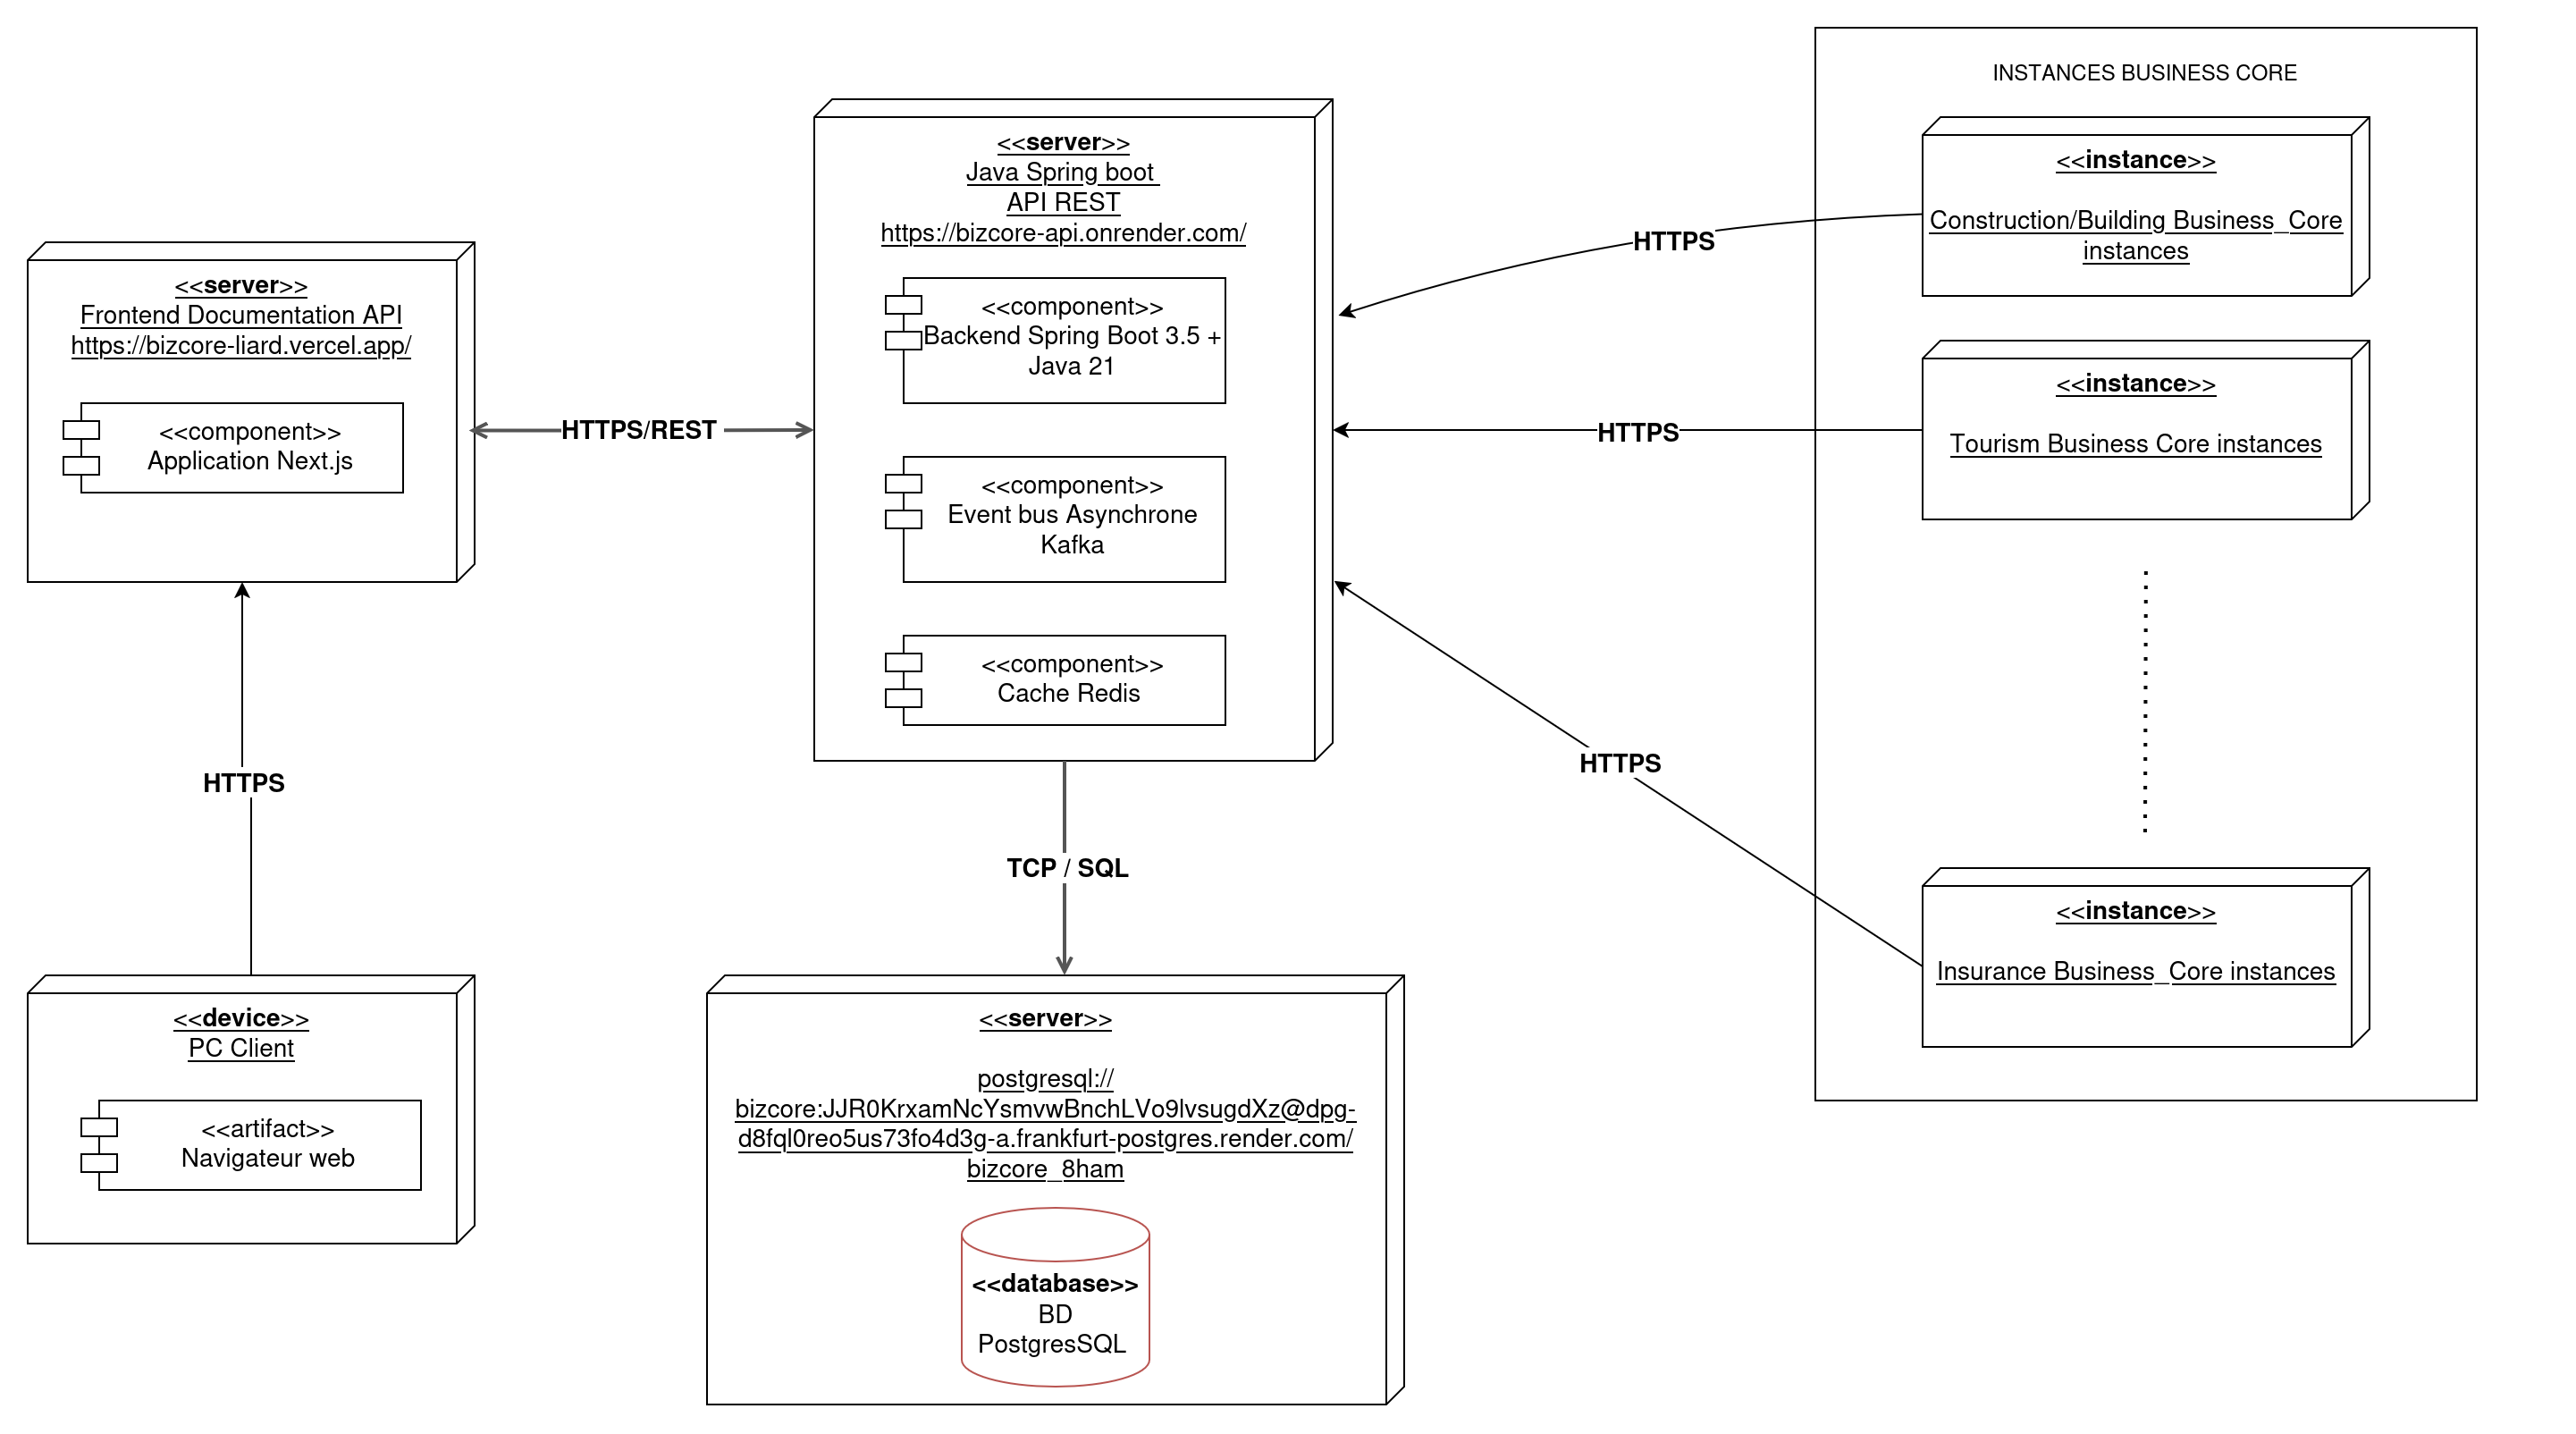
\includegraphics[width=\linewidth]{figures/diagrammes/DEPLOIEMENT.drawio.png}
   \captionof{figure}{Diagramme de déploiement du système}
    \label{fig:deploy}
\end{figure}
\label{fig:deploy} 

\begin{figure}[htbp]
  \centering
  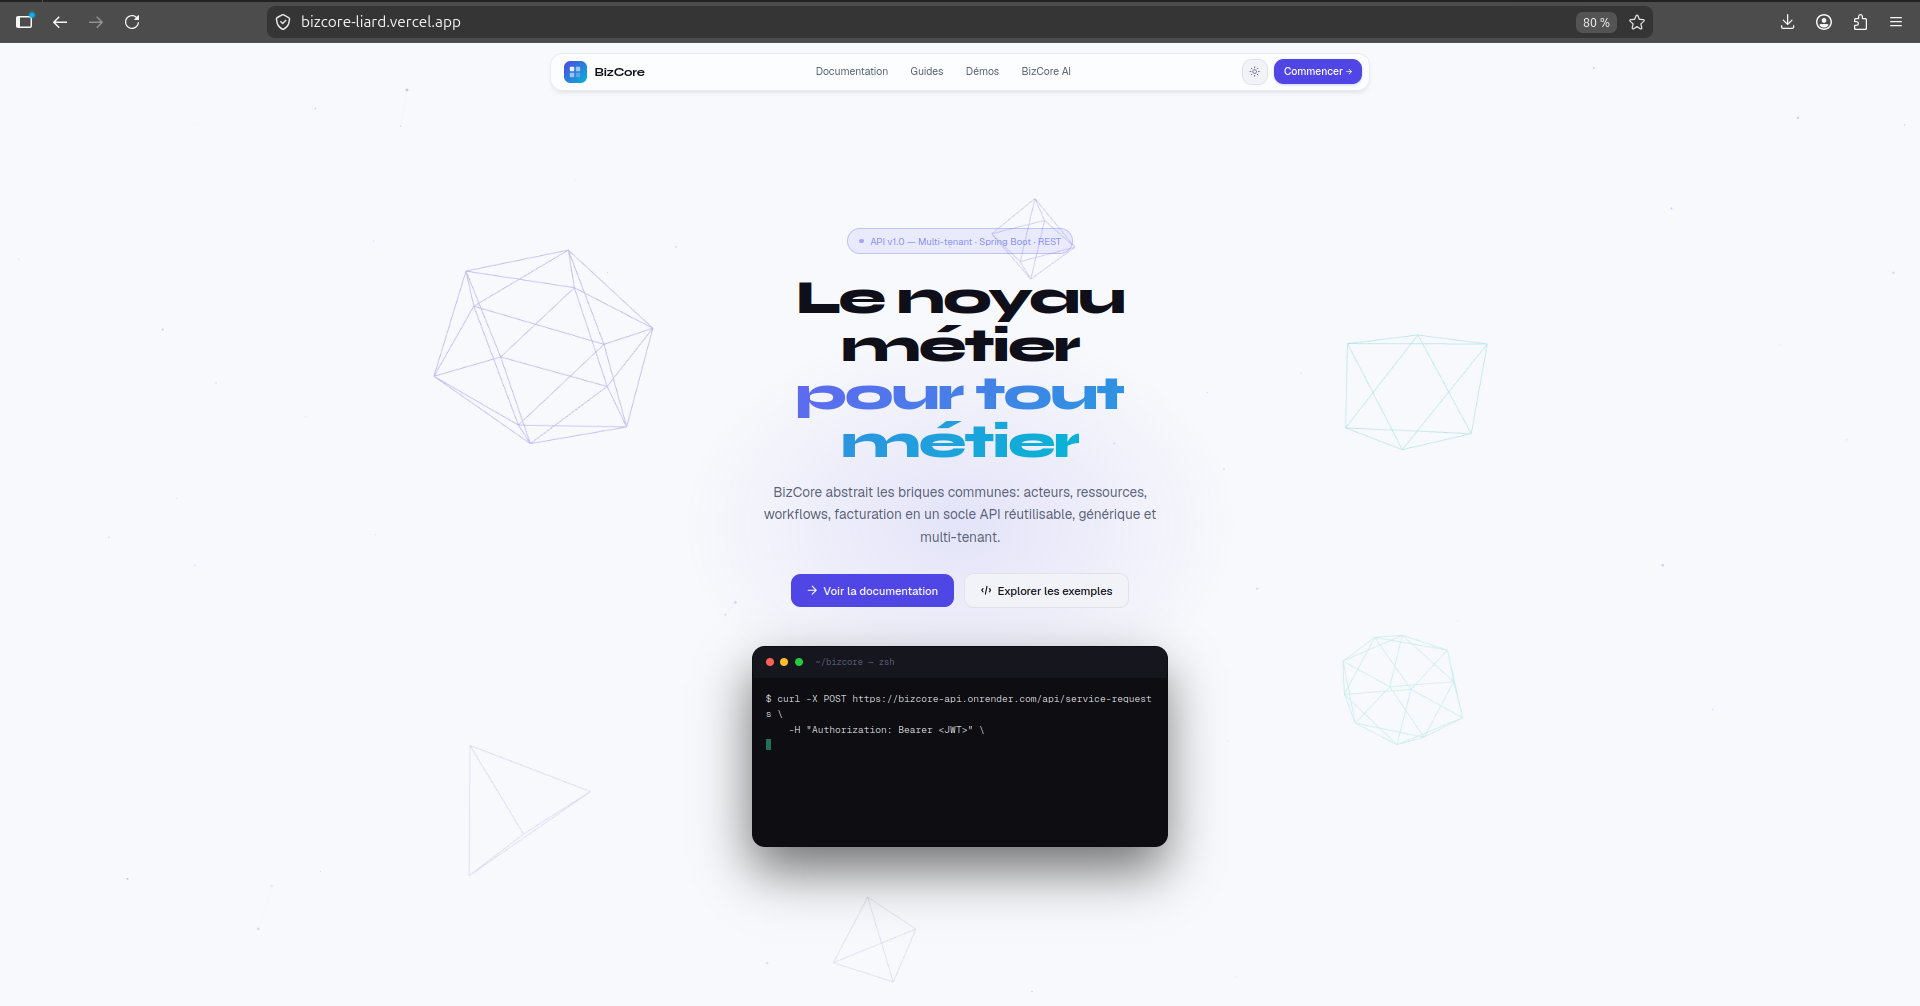
\includegraphics[width=0.95\textwidth]{figures/Screenshots/VITRINE.png}
  \caption{Page d'accueil du site vitrine déployé sur Vercel}
  \label{fig:front-home}
\end{figure}

\begin{figure}[htbp]
  \centering
  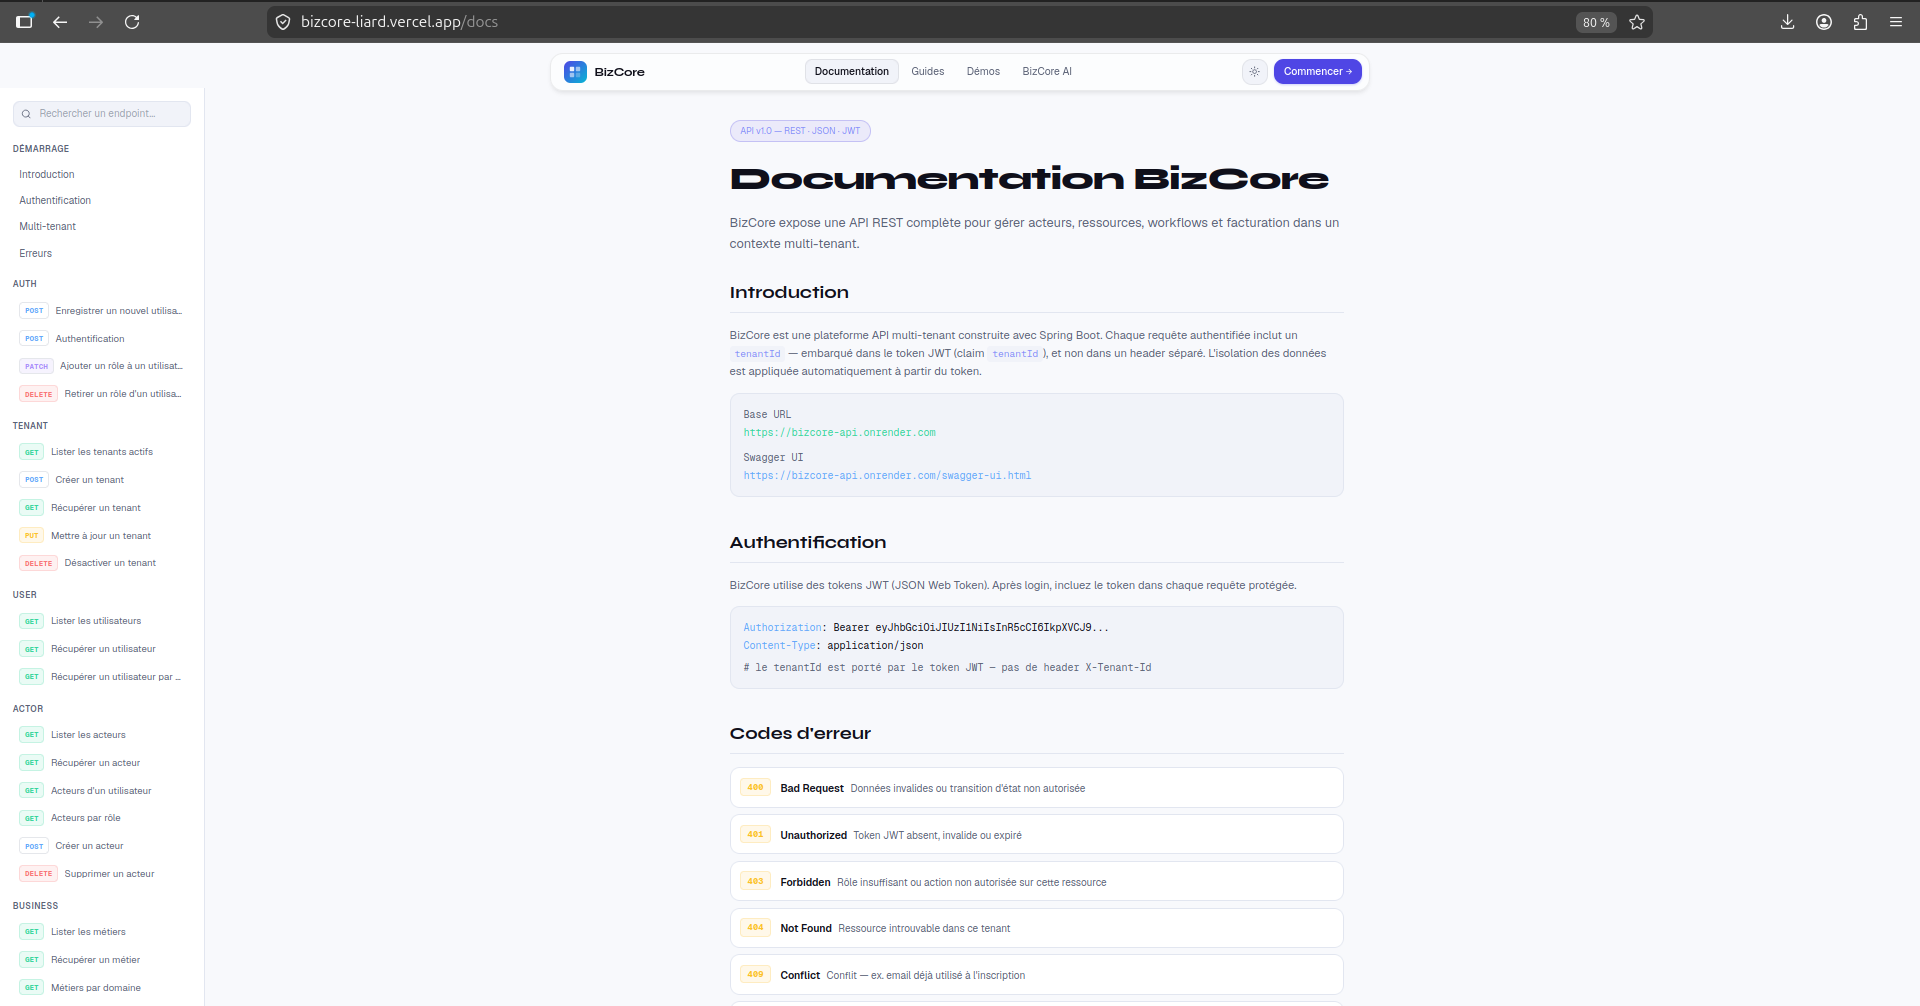
\includegraphics[width=0.95\textwidth]{figures/Screenshots/DOCUMENTATION.png}
  \caption{Documentation interactive de l'API}
  \label{fig:front-docum}
\end{figure}
 